\documentclass{sigchi}

% Use this section to set the ACM copyright statement (e.g. for
% preprints).  Consult the conference website for the camera-ready
% copyright statement.

% Copyright
\CopyrightYear{2017}
%\setcopyright{acmcopyright}
\setcopyright{acmlicensed}
%\setcopyright{rightsretained}
%\setcopyright{usgov}
%\setcopyright{usgovmixed}
%\setcopyright{cagov}
%\setcopyright{cagovmixed}
% DOI
\doi{http://dx.doi.org/10.475/123_4}
% ISBN
\isbn{123-4567-24-567/08/06}
%Conference
\conferenceinfo{HAI'17,}{October 17--20, 2016, Bielefeld, Germany}
%Price
\acmPrice{\$15.00}

% Use this command to override the default ACM copyright statement
% (e.g. for preprints).  Consult the conference website for the
% camera-ready copyright statement.

%% HOW TO OVERRIDE THE DEFAULT COPYRIGHT STRIP --
%% Please note you need to make sure the copy for your specific
%% license is used here!
% \toappear{
% Permission to make digital or hard copies of all or part of this work
% for personal or classroom use is granted without fee provided that
% copies are not made or distributed for profit or commercial advantage
% and that copies bear this notice and the full citation on the first
% page. Copyrights for components of this work owned by others than ACM
% must be honored. Abstracting with credit is permitted. To copy
% otherwise, or republish, to post on servers or to redistribute to
% lists, requires prior specific permission and/or a fee. Request
% permissions from \href{mailto:Permissions@acm.org}{Permissions@acm.org}. \\
% \emph{CHI '16},  May 07--12, 2016, San Jose, CA, USA \\
% ACM xxx-x-xxxx-xxxx-x/xx/xx\ldots \$15.00 \\
% DOI: \url{http://dx.doi.org/xx.xxxx/xxxxxxx.xxxxxxx}
% }

% Arabic page numbers for submission.  Remove this line to eliminate
% page numbers for the camera ready copy
% \pagenumbering{arabic}

% Load basic packages
\usepackage{balance}       % to better equalize the last page
\usepackage{graphics}      % for EPS, load graphicx instead
\usepackage[T1]{fontenc}   % for umlauts and other diaeresis
\usepackage{txfonts}
\usepackage{mathptmx}
\usepackage[pdflang={en-US},pdftex]{hyperref}
\usepackage{color}
\usepackage{booktabs}
\usepackage{textcomp}

% Some optional stuff you might like/need.
\usepackage{microtype}        % Improved Tracking and Kerning
% \usepackage[all]{hypcap}    % Fixes bug in hyperref caption linking
\usepackage{ccicons}          % Cite your images correctly!
% \usepackage[utf8]{inputenc} % for a UTF8 editor only

% If you want to use todo notes, marginpars etc. during creation of
% your draft document, you have to enable the "chi_draft" option for
% the document class. To do this, change the very first line to:
% "\documentclass[chi_draft]{sigchi}". You can then place todo notes
% by using the "\todo{...}"  command. Make sure to disable the draft
% option again before submitting your final document.
\usepackage{todonotes}

\usepackage{eurosym}

% Paper metadata (use plain text, for PDF inclusion and later
% re-using, if desired).  Use \emtpyauthor when submitting for review
% so you remain anonymous.
% \def\plaintitle{SIGCHI Conference Proceedings Format}
\def\plaintitle{Towards the Analysis of Movement Variability in Human-Humanoid
Imitation Activities}

\def\plainauthor{First Author, Second Author, Third Author,
  Fourth Author, Fifth Author, Sixth Author}
\def\emptyauthor{}
\def\plainkeywords{Authors' choice; of terms; separated; by
  semicolons; include commas, within terms only; required.}
\def\plaingeneralterms{Documentation, Standardization}

% llt: Define a global style for URLs, rather that the default one
\makeatletter
\def\url@leostyle{%
  \@ifundefined{selectfont}{
    \def\UrlFont{\sf}
  }{
    \def\UrlFont{\small\bf\ttfamily}
  }}
\makeatother
\urlstyle{leo}

% To make various LaTeX processors do the right thing with page size.
\def\pprw{8.5in}
\def\pprh{11in}
\special{papersize=\pprw,\pprh}
\setlength{\paperwidth}{\pprw}
\setlength{\paperheight}{\pprh}
\setlength{\pdfpagewidth}{\pprw}
\setlength{\pdfpageheight}{\pprh}

% Make sure hyperref comes last of your loaded packages, to give it a
% fighting chance of not being over-written, since its job is to
% redefine many LaTeX commands.
\definecolor{linkColor}{RGB}{6,125,233}
\hypersetup{%
  pdftitle={\plaintitle},
% Use \plainauthor for final version.
%  pdfauthor={\plainauthor},
  pdfauthor={\emptyauthor},
  pdfkeywords={\plainkeywords},
  pdfdisplaydoctitle=true, % For Accessibility
  bookmarksnumbered,
  pdfstartview={FitH},
  colorlinks,
  citecolor=black,
  filecolor=black,
  linkcolor=black,
  urlcolor=linkColor,
  breaklinks=true,
  hypertexnames=false
}

% create a shortcut to typeset table headings
% \newcommand\tabhead[1]{\small\textbf{#1}}

% End of preamble. Here it comes the document.
\begin{document}

\title{\plaintitle}

\numberofauthors{3}
\author{%
  \alignauthor{Leave Authors Anonymous\\
    \affaddr{for Submission}\\
    \affaddr{City, Country}\\
    \email{e-mail address}}\\
  \alignauthor{Leave Authors Anonymous\\
    \affaddr{for Submission}\\
    \affaddr{City, Country}\\
    \email{e-mail address}}\\
}

\maketitle


\begin{abstract}
  In this paper, we present preliminary results for the analysis of movement
  variability in order to quantify face-to-face human-humanoid imitation activities.
  We applied the state space reconstruction's theorem to test our
  hypothesis where participants, even performing the same arm movement,
  presented minor difference in the way they moved.
  With this in mind, we asked eighteen participants to copy NAO's arm
  movements while we collected data from inertial sensors attached to the
  participants' wrist and estimated the head pose using the OpenFace framework.
  With the proposed metric, we found that two participants were moving their arms
  asymmetrically while others move their arms symmetrically.
  We also showed that two participants where moving
  their head even when NAO's head was static.
  Although the work is in its early stage, the results are promising for
  applications in rehabilitation, sport science, entertainment or education.
\end{abstract}

\category{I.2.9.}{Robotics}{Sensors}
\category{G.3.}{PROBABILITY AND STATISTICS}{Time series analysis}
% \category{I.5.4.}{Applications}{Signal Progessing}

% \keywords{\plainkeywords}
\keywords{Human-Robot Interaction; Human-Humanoid Imitation;
Wearable Inertial Sensors; State Space Reconstruction; Nonlinear dynamics;
Dynamics Invariants}


\section{Introduction}

Movement variability is an inherent feature within a person and between persons
movements \cite{newell1993variability}. Recently, Herzfeld et al. \cite{Herzfeld2014}
conducted experiments to state that movement variability is not only noise but a
source of movement exploration which at certain point of the exploration
such variability is becoming a source of movement exploration.
With this in mind, we have found that there is little research in the area of
human-robot interaction that is focused on the quantification of movement variability.

The paper is divided into an intuitive explanation of the state space reconstruction,
experiment design, results and conclusions.



\section{METHOD}

\subsection{State Space Reconstruction's Theorem}
The purpose of the State Space Reconstruction's Theorem, also known as
time-delay embedding, is to reconstruct the topological properties of an
unknown $M-$dimensional state space $s(t)$ from a $1-$dimensional measurement
$x(t)$ in order to reconstruct an $N-$dimensional embedding space
(Figure \ref{fig:takens_theorem}).
%%---------------------------------(FIGURE)-------------------------------------
% \begin{figure}[!htb]
\begin{figure}
\centering
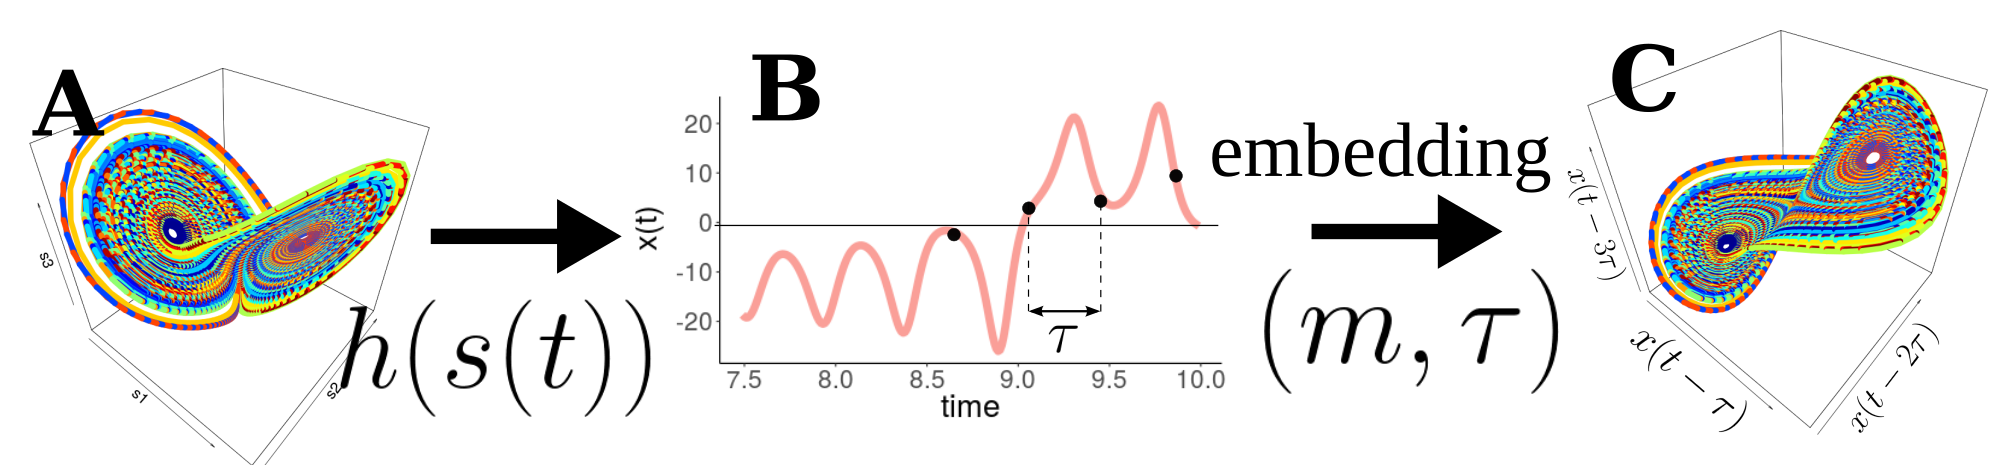
\includegraphics[width=0.45\textwidth]{figures/reconstructed_state_space/fig_v01}
\caption[PA]{State Space Reconstruction. A. $M-$dimensional state space $s(t)$;
B. $1-$dimensional measurement time-series $x(t)$; and
C. $N-$dimensional reconstructed state space $v(t)$
where $M \geq N$ (adapted from \cite{QuintanaDuque2012}).}
\label{fig:takens_theorem}
\end{figure}
%%---------------------------------(FIGURE)-------------------------------------
The time-delay embedding assumes that the time-series is a sequence $x(t)=h(s(t))$,
where $h: S \rightarrow \mathbb{R}^M$ is a measurement function on the unknown
dynamical system, being $x(t)$ observable.
Thus, the time delay reconstruction in $m$ dimensions with a time delay
$\tau$ is defined as: $\overline{x}(t) = (x(t), x(t-\tau),...,x(t-(m-1)\tau))$.
Then a further transformation is considered, e.g. PCA, in order to reduce
the dimensionality of the $m-$dimensional reconstructed state space
to a $k-$dimensional space \cite{Uzal2011}.
For this work, we assume that the signal, $x(t)$, is produced by some time-varying
system in our case the time-series are produced by the linear acceleration of
the inertial sensors.
We assume that the time-series, over some time period, exhibit a systematic
variability between and within persons movements.
What we do not know is how reliable the quantification methods for movement variability are
and how the levels of imitation of a given range of movement variability can be established.


\subsection{Determining the embedding parameters ($m$ and $\tau$)}
Although State Space Reconstruction's Theorem has been used extensively in gait
recognition and walking, running and cycling activities \cite{Frank2010,Sama2013},
the computation of the minimal embedding parameters largely depend on the
structure of the time-series (amplitude, frequency, nonlinearity).
To which, we however first compute the minimal embedding parameters
using the Cao's algorithm \cite{Cao1997} and the mutual information
and then we manually increase the dimensionality of the reconstructed state
space until the attractor is untangled.

\section{Experiment Design}

\subsection{Measuring Movement}
To understand the movement variability of the participants, we use
four Wearable Inertial Sensors SEN-10736 SparkFun 9DOF RAZOR
with triple-axis accelerometer and triple-axis gyroscope (Figure~\ref{fig:exp}A).
The data were transmitted via RN42 bluetooth module
for which we set a sampling rate of 50 Hz and collected using ROS \cite{quigley2009}.

\subsection{Time-series from the Accelerometer Sensor}
The sequences ($a_x(n),a_y(n),a_z(n)$) are the raw data collected from the
triaxial accelerometer sensor. Then, for instance, the time-series $a_x(n)$
with a length of $N$ samples is employed to get the embedded state space matrix,
$\boldsymbol{E} a_{x}$, with $m$ rows and $N-(m-1)\tau$ columns.
PCA is then applied to reduce de dimensionality of the data choosing the first
two components of the rotated data in order to reconstruct the state space.


\subsection{Head Pose Estimation}
Estimating head pose in human-robot interactions is an active area of research
where challenges like real-time tracking, the use of less invasive equipment
or the long-time preparation of calibration techniques of the motion capture
systems remain to be solved. Recently, Lemaignan et al. \cite{Lemaignan2016}
proposed a head pose estimator using a monocular RGB webcam which is able to
track a head with rotations up to $\pm$40$^{\circ}$ horizontally and
$\pm$30$^{\circ}$ vertically.
However, OpenFace, a fully open source real-time facial behaviour analysis,
non only provides head pose (orientation and motion) but also a state-of-the-art
performance in facial landmark motion, facial expressions, and eye gaze
\cite{Baltrusaitis2016}.
We therefore select the OpenFace because of the simple set up, less invasive and
the features for face behaviour, besides it can operate with a simple webcam in
real-time (Figure~\ref{fig:exp}B).

\section{Experiment}

\subsection{Hypothesis}
In our previous experiments of a face-to-face human-humanoid imitation
activity \cite{XXX2017}, we applied the State Space Reconstruction's Theorem
to quantify the level of imitation for horizontal and vertical upper arm movements.
In such experiment, we observed in the recorded videos that the effects like
boredom, fatigue or level of engagement play an important role in the influence
that each persons moves.
With this in mind, we hypothesised that not only the inertial sensors attached
to the body can provide information about movement variability but also the
face expressions and head pose estimation which, we believe, will lead us
to get better understanding of the movement variability in human-to-humanoid
activities and therefore create more reliable metrics to quantify such variability.


\subsection{Participants and Procedure}
To test our hypothesis, we collected data from eighteen healthy participants:
eight male participant (age 18 $\pm$ 3.43) and ten female (age 18 $\pm$ 0.43)
in which inertial sensors were attached to the wrist of both the participant and the
humanoid robot, and put the webcam in front of the participant for the head pose
estimation (Figure~\ref{fig:exp}A).
In the experiment, participant were asked to imitate NAO's upper arm movements
with ten repetitions (Figure~\ref{fig:nao}).
%%---------------------------------(FIGURE)-------------------------------------
% \begin{figure}[!htb]
\begin{figure}
\centering
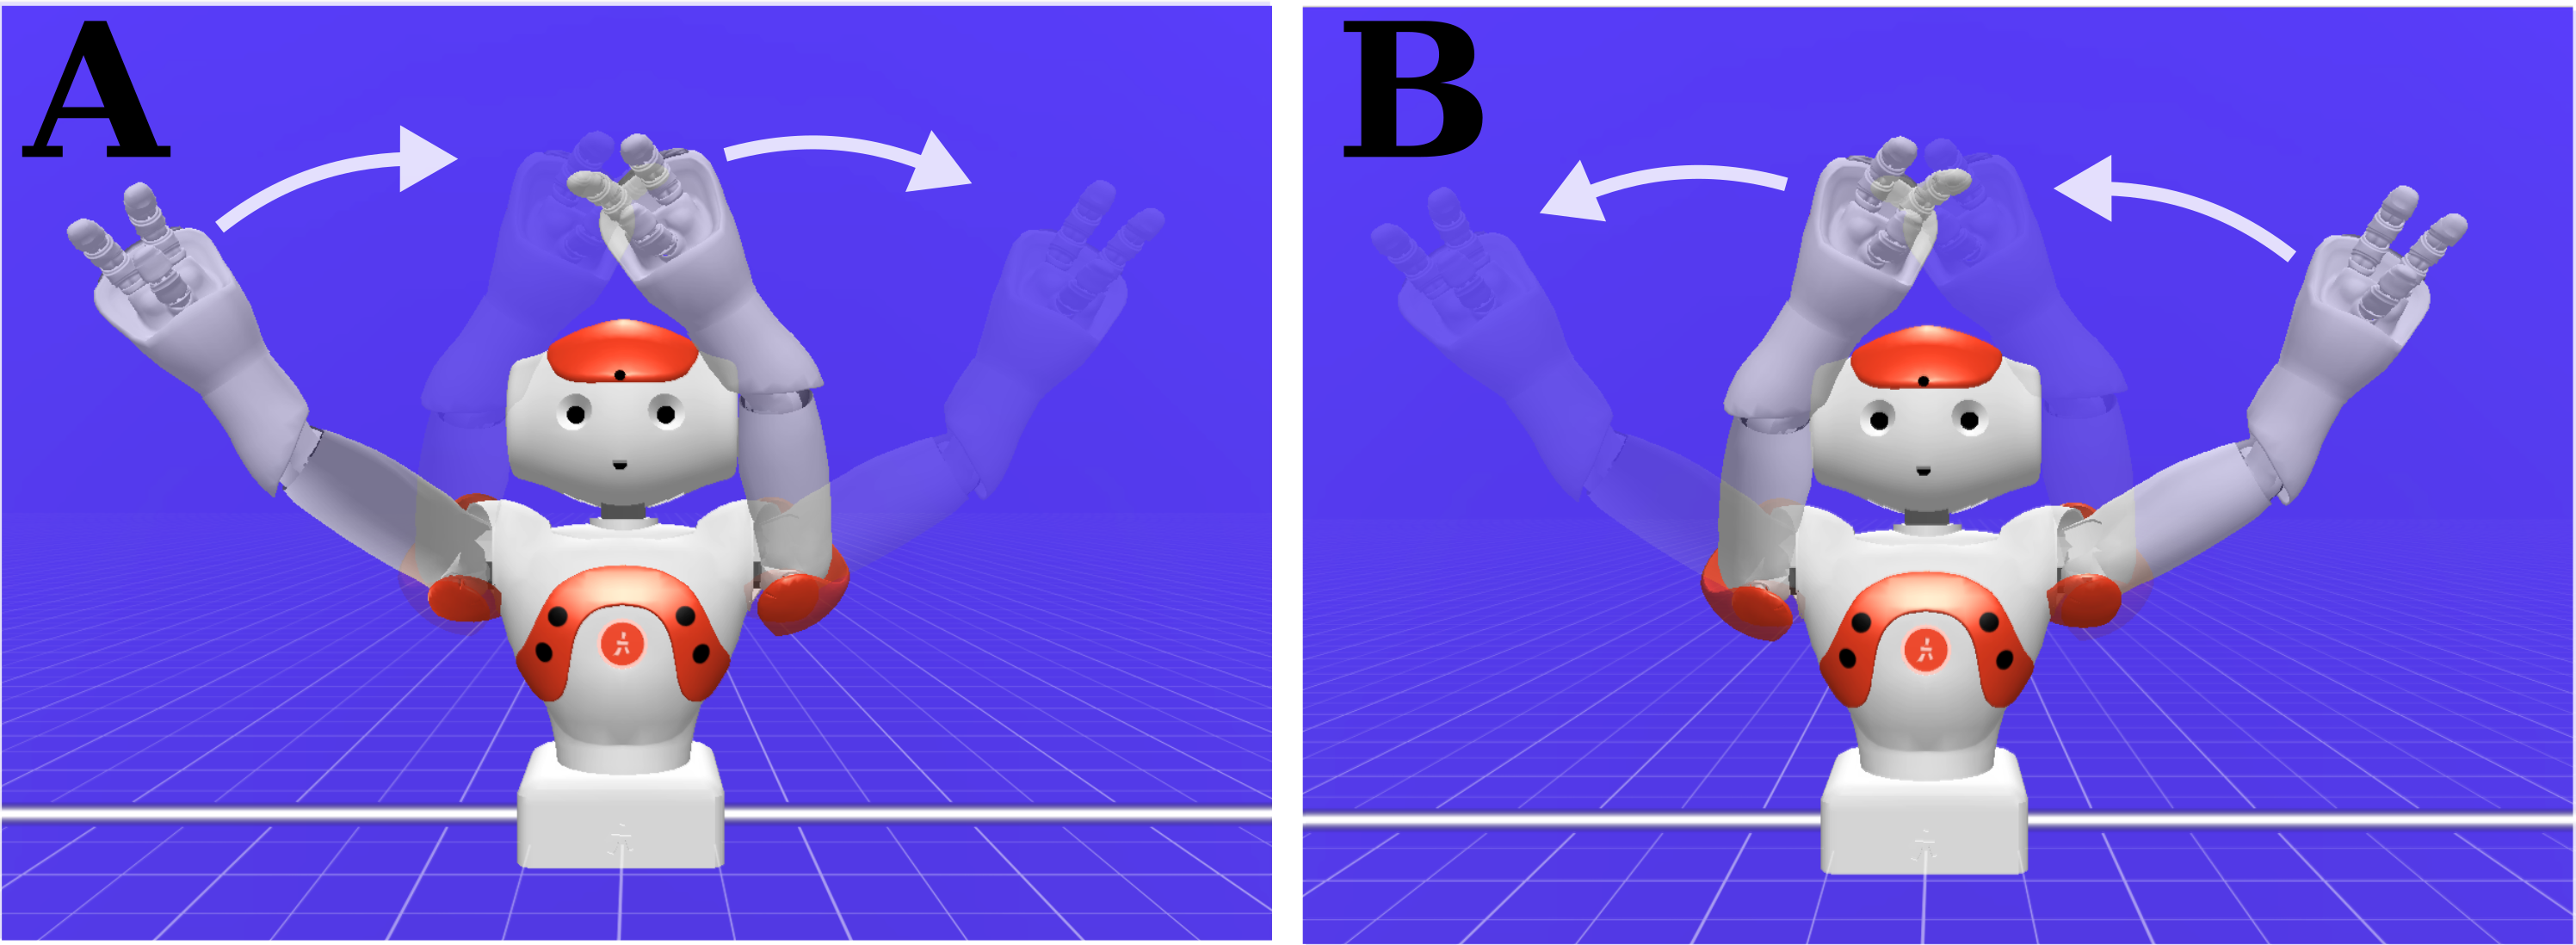
\includegraphics[width=0.45\textwidth]{figures/nao/arm_movements/fignao}
\caption[PA]{NAO's arm movements. A. Moving arms from right to left;
B. Moving arms from left to right.  }
\label{fig:nao}
\end{figure}
%%---------------------------------(FIGURE)-------------------------------------
%%---------------------------------(FIGURE)-------------------------------------
% \begin{figure}[!htb]
\begin{figure}
\centering
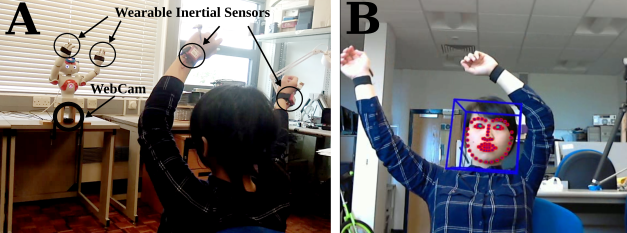
\includegraphics[width=0.45\textwidth]{figures/experiment/fig_w619h233_v2}
\caption[PA]{A. Experimental set-up: face-to-face imitation with NAO humanoid robot;
B. Head pose estimation with OpenFace \cite{Baltrusaitis2016} }
\label{fig:exp}
\end{figure}
%%---------------------------------(FIGURE)-------------------------------------
\section{Results}
In Figure~\ref{fig:main}A, we only presented time-series for the participant 12
for the sensors attached to the right and left wrist (red and blue).
With this in mind, we showed that the asymmetry of the signals which is
reflected in p12-sLeft and p12-sRight in (Figure~\ref{fig:main}B) as well as in the
error plot (Figure~\ref{fig:main}C).
For the error bars of the OpenFace, you can notice the well distributed
data in the interquartile range for participants p04 and p17 (Figure~\ref{fig:main}C)
which means that those participants were moving their heads as their hands.
The expanded distribution of the interquartile range for participant p14
means that p14 head's movement was quite static.
\begin{figure*}[!htb]
\centering
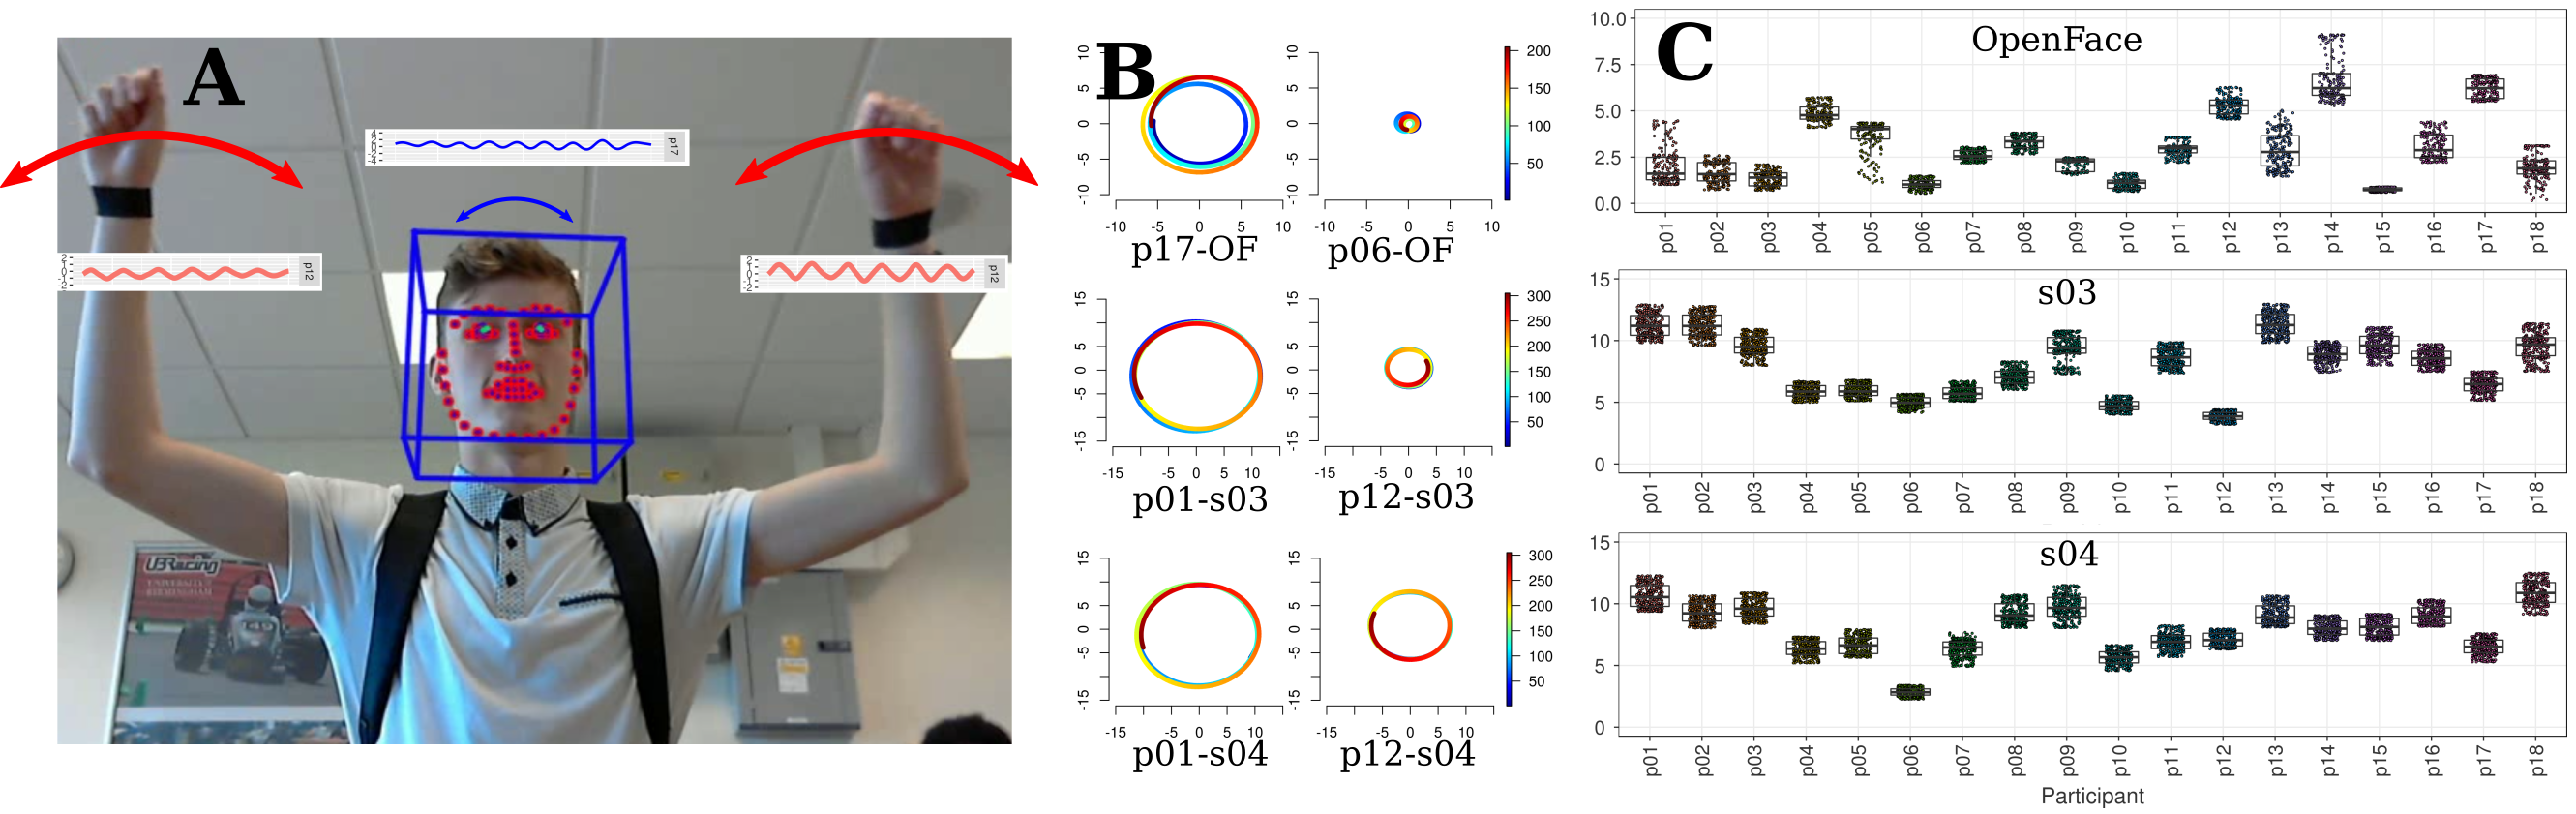
\includegraphics[width=1.00\textwidth]{figures/results/main/figv01}
\caption[PA]{
A. time-series for the inertial sensors $a_x(n)$ and the
Head Pose Estimation in the $T_x$ axis;
B. State Space Reconstruction with $m=100$ and $\tau=4$ for
participants 17 and 16 for the head pose estimation and
participants 01 and 12 for sensor 03 and 04;
C. Error bars for the head pose estimation, sensor 03 and sensor 04 for
the eighteen participants.}
\label{fig:main}
\end{figure*}


\section{Conclusion}


Having proposed the use of the state space reconstruction to analyse human-humanoid
imitation activity, several questions remain to be investigated such as the
understanding of variability of emotions and motions in one-to-one or
one-to-many human-humanoid interactions.
Considering the fact that the robot's head was static in the activity,
we observed that the interquartile range of the proposed metric for participants p04 and p17
is an indication of the movement of their heads as a tendency for the arm movements.
We believe that such behaviour requires further investigation for which the motor
experience affects the visual sensitivity of human action \cite{blake2007}.

In future experiments, there are four areas that we intend to investigate:
(a) performance of experiments of not only one-to-one interaction but
two-humans to one-humanoid and three-humans to one-humanoid interactions;
(b) exploration of complex movements which can be performed by both persons and NAO;
(c) data collection from a wider range of individuals
(different gender, age and state of health) and from additional inertial sensors
attached to the body; and
(d) application of deep learning techniques to automatically classify the
movement variability.



\section{Acknowledgments}

XXX gratefully acknowledges XXX for funding his doctoral studies at
University of XXX.

% Balancing columns in a ref list is a bit of a pain because you
% either use a hack like flushend or balance, or manually insert
% a column break.  http://www.tex.ac.uk/cgi-bin/texfaq2html?label=balance
% multicols doesn't work because we're already in two-column mode,
% and flushend isn't awesome, so I choose balance.  See this
% for more info: http://cs.brown.edu/system/software/latex/doc/balance.pdf
%
% Note that in a perfect world balance wants to be in the first
% column of the last page.
%
% If balance doesn't work for you, you can remove that and
% hard-code a column break into the bbl file right before you
% submit:
%
% http://stackoverflow.com/questions/2149854/how-to-manually-equalize-columns-
% in-an-ieee-paper-if-using-bibtex
%
% Or, just remove \balance and give up on balancing the last page.
%
% \balance{}


% BALANCE COLUMNS
\balance{}

% REFERENCES FORMAT
% References must be the same font size as other body text.
\bibliographystyle{SIGCHI-Reference-Format}
\bibliography{references}

\end{document}

%%% Local Variables:
%%% mode: latex
%%% TeX-master: t
%%% End:
